\documentclass{article}

% Language setting
% Replace `english' with e.g. `spanish' to change the document language
\usepackage[english]{babel}
\usepackage[table,xcdraw]{xcolor}
\usepackage{float}
\usepackage[backend=biber,style=apa]{biblatex}
\addbibresource{reference.bib}
\addbibresource{rpackage.bib}

% Set page size and margins
% Replace `letterpaper' with `a4paper' for UK/EU standard size
\usepackage[letterpaper,top=2cm,bottom=2cm,left=3cm,right=3cm,marginparwidth=1.75cm]{geometry}

% Useful packages
\usepackage{amsmath}
\usepackage{graphicx}
\usepackage[colorlinks=true, allcolors=blue]{hyperref}

\title{Final Project}
\author{Xinyi Yu}

\begin{document}
\maketitle

\section{Introduction}

The dataset analyzed in this project was derived from the study of \cite{overmyer_large-scale_2021}, which profiled immune responses in COVID-19 patients and non-COVID controls. For the main analyses, we focus on the AAAS gene. The AAAS gene encodes a member of the WD-repeat family of regulatory proteins, which is part of the nuclear pore complex and anchored by NDC1. It plays an important role in the development of the peripheral and central nervous system. Mutations in this gene cause achalasia-addisonianism-alacrima syndrome (AAAS), also known as triple-A or Allgrove syndrome \cite{pubchem_aaas_nodate}. Given its role in nuclear pore complex function and stress response, AAAS was selected as a candidate gene for this analysis due to its potential relevance for host-pathogen interactions and immune dysregulation in COVID-19.


\section{Methods}

\subsection{Data Source}

The dataset was obtained from the study by \cite{overmyer_large-scale_2021}, available through public repositories associated with the publication.

\subsection{R Version and Packages}

The analyses were conducted in R version 4.2.1. The main packages included tidyverse \cite{tidyverse2019} for data manipulation and visualization, ggplot2 \cite{ggplot22016} for plotting, pheatmap \cite{pheatmap2025} for heatmap generation, and kableExtra \cite{kableExtra2021} for creating and formatting complex tables.

\subsection{Clustering algorithm}

Hierarchical clustering was performed on the gene expression data using the Euclidean distance and complete linkage to generate the heatmap.

\section{Results}

\subsection{Table 1. Summary statistics by disease status}

Table 1 shows the summary statistics by disease status. Continuous variables are summarized as mean with standard deviation and categorical variables as counts with percentages. Patients with COVID-19 tend to be older and have higher ferritin levels, and ICU cases are more common in this group. The sex distribution is relatively balanced. In general, the COVID-19 group appears clinically more severe, and future work can test whether these observed differences are statistically significant.

\begin{table}[H]
\centering
\caption{\label{tab:summary}Summary statistics by disease status}
\begin{tabular}{llll}
\hline
{\color[HTML]{222222} Variable} &
  {\color[HTML]{222222} disease state: COVID-19} &
  {\color[HTML]{222222} disease state: non-COVID-19} &
  {\color[HTML]{222222} Overall} \\ \hline
{\color[HTML]{222222} age} &
  {\color[HTML]{222222} 60.84 (16.15)} &
  {\color[HTML]{222222} 61.96 (15.36)} &
  {\color[HTML]{222222} 61.06 (15.94)} \\
{\color[HTML]{222222} hospital\_free} &
  {\color[HTML]{222222} 22.09 (16.62)} &
  {\color[HTML]{222222} 32.36 (15.09)} &
  {\color[HTML]{222222} 24.14 (16.79)} \\
{\color[HTML]{222222} ferritin} &
  {\color[HTML]{222222} 932.76 (1094.04)} &
  {\color[HTML]{222222} 250.50 (238.21)} &
  {\color[HTML]{222222} 833.52 (1042.80)} \\
{\color[HTML]{222222} sex}         & {\color[HTML]{222222} -}           & {\color[HTML]{222222} -}           & {\color[HTML]{222222} -} \\
{\color[HTML]{222222} female}      & {\color[HTML]{222222} 38 (38.0\%)} & {\color[HTML]{222222} 13 (52.0\%)} & {\color[HTML]{222222} -} \\
{\color[HTML]{222222} male}        & {\color[HTML]{222222} 62 (62.0\%)} & {\color[HTML]{222222} 12 (48.0\%)} & {\color[HTML]{222222} -} \\
{\color[HTML]{222222} icu\_status} & {\color[HTML]{222222} -}           & {\color[HTML]{222222} -}           & {\color[HTML]{222222} -} \\
{\color[HTML]{222222} no}          & {\color[HTML]{222222} 50 (50.0\%)} & {\color[HTML]{222222} 10 (40.0\%)} & {\color[HTML]{222222} -} \\
{\color[HTML]{222222} yes}         & {\color[HTML]{222222} 50 (50.0\%)} & {\color[HTML]{222222} 15 (60.0\%)} & {\color[HTML]{222222} -} \\ \hline
\end{tabular}
\end{table}

\subsection{Histogram of Gene Expression}

The histogram shows the distribution of AAAS expression levels in all samples. The x-axis represents AAAS expression levels, and the y-axis represents the number of samples. Expression values appear to be approximately symmetric, with most samples clustered between 10 and 20. This suggests that while there is variability, extreme high or low expression values are uncommon.

\begin{figure}[H]
\centering
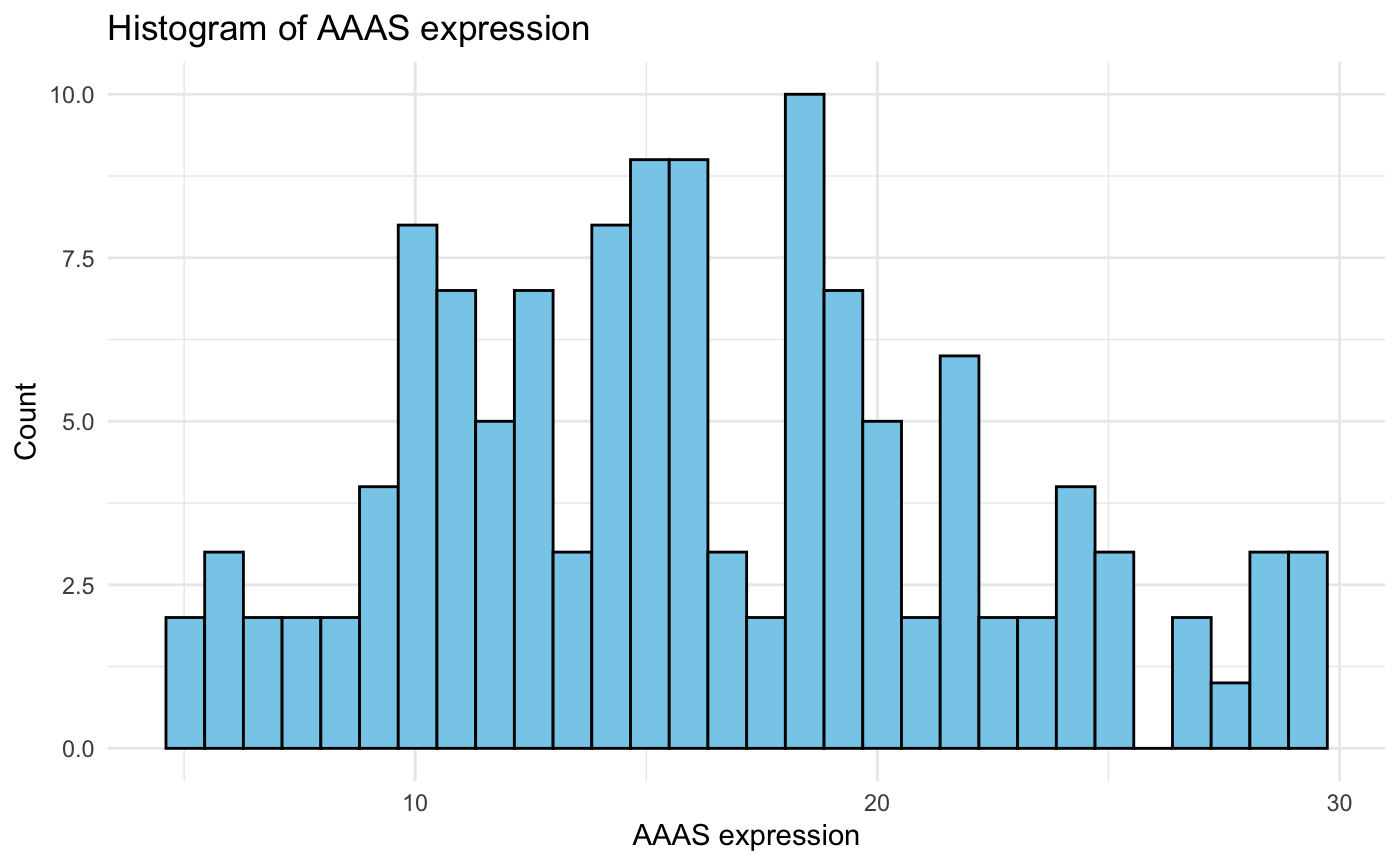
\includegraphics[width=0.80\linewidth]{Histogram of AAAS expression.png}
\caption{\label{fig:histogram}Histogram of Gene Expression}
\end{figure}

\subsection{Scatter Plot of Gene Expression vs Age}

The scatter plot illustrates the relationship between AAAS expression and age. Each point represents a sample. No clear linear association was observed, as the expression values appear scattered between age groups. This suggests that age alone may not strongly influence AAAS expression.

\begin{figure}[H]
\centering
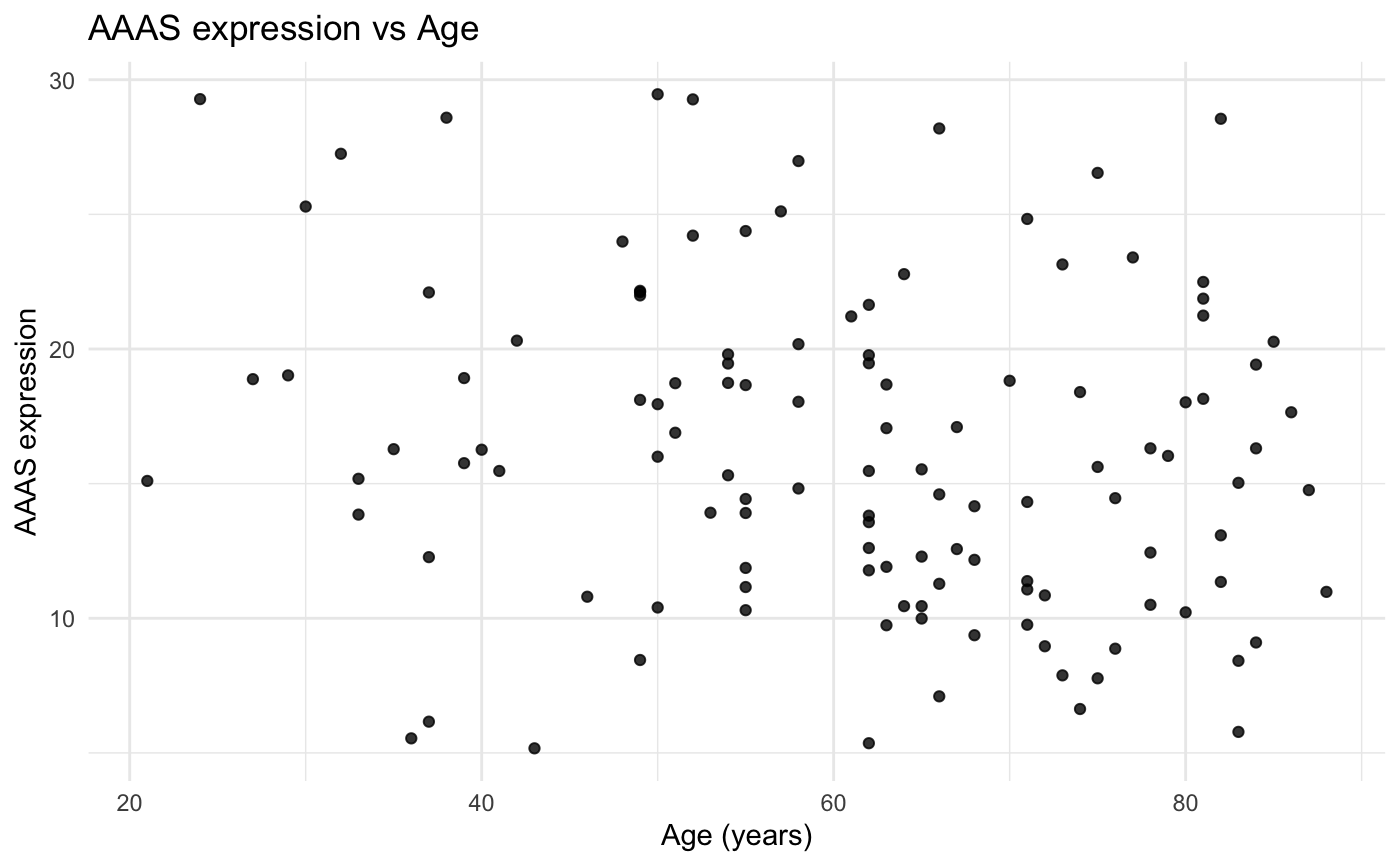
\includegraphics[width=0.80\linewidth]{AAAS expression vs Age.png}
\caption{\label{fig:scatterplot}Scatter Plot of Gene Expression vs Age}
\end{figure}

\subsection{Boxplot of gene stratified by 2 categorical covariates}

This boxplot shows how AAAS expression varies by sex and disease status. The x-axis shows biological sex and colors indicate disease state. For both females and males, COVID-19 patients tend to show higher variability and slightly higher median expression. Non-COVID samples have more compact expression ranges. Among males, COVID-19 patients have a higher median expression of AAAS than Non-Covid 19 patients. All above might implies that neither sex nor disease status alone explains differences in AAAS expression, but interactions could be further explored.

\begin{figure}[H]
\centering
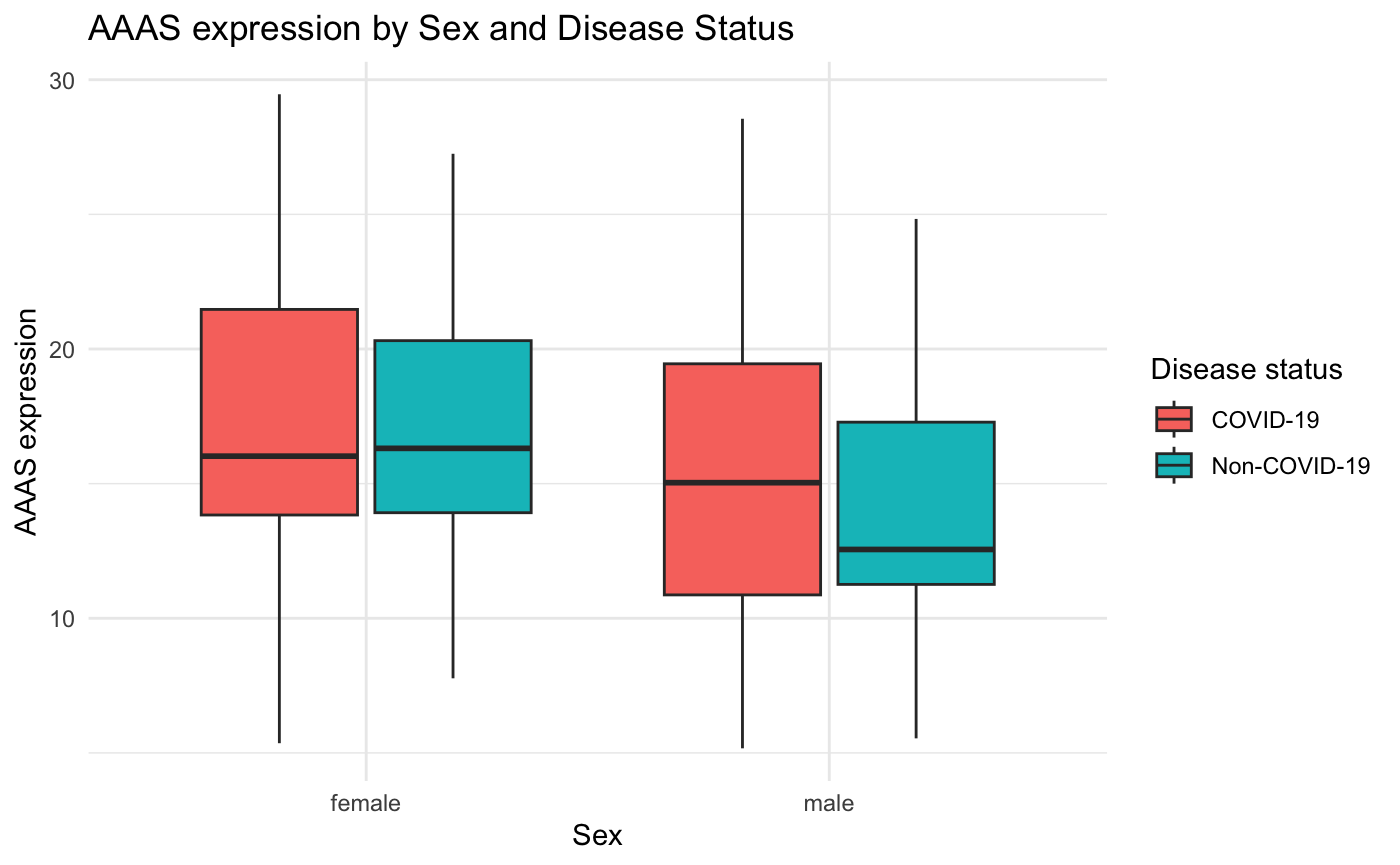
\includegraphics[width=0.80\linewidth]{AAAS expression by Sex and Disease Status.png}
\caption{\label{fig:boxplot}Boxplot of AAAS gene expression stratified by sex and disease status}
\end{figure}

\subsection{Heatmap of top variable genes}

This heatmap shows the expression of 20 genes with the largest variance in 20 randomly sampled samples. Red indicates higher expression (after log2 transformation), blue indicates lower expression, and yellow indicates intermediate levels. Genes with similar expression patterns are grouped together. For example, ABCG1 shows low expression in most samples and is clustered with other low-expression genes such as ABHD13 and ABCC5. In contrast, ABHD3, ABHD5, and ABHD16A show much higher expression in some samples and are clustered together. The clustering of samples does not separate COVID-19 from non-COVID-19 or males from females. Instead, samples from different groups are mixed, which suggests that disease status and sex are not the main factors here. Some genes, such as ABHD3, also show strong variation between individuals, with some samples very high (dark red) and others much lower (light blue). This variation looks stronger than the effect of disease status or sex. In conclusion, the heatmap highlights two main patterns: one cluster of genes with consistently low expression, and another with variable or high expression peaks. Clinical variables do not drive the clustering, while individual differences and gene-specific behavior play a stronger role.

\begin{figure}[H]
\centering
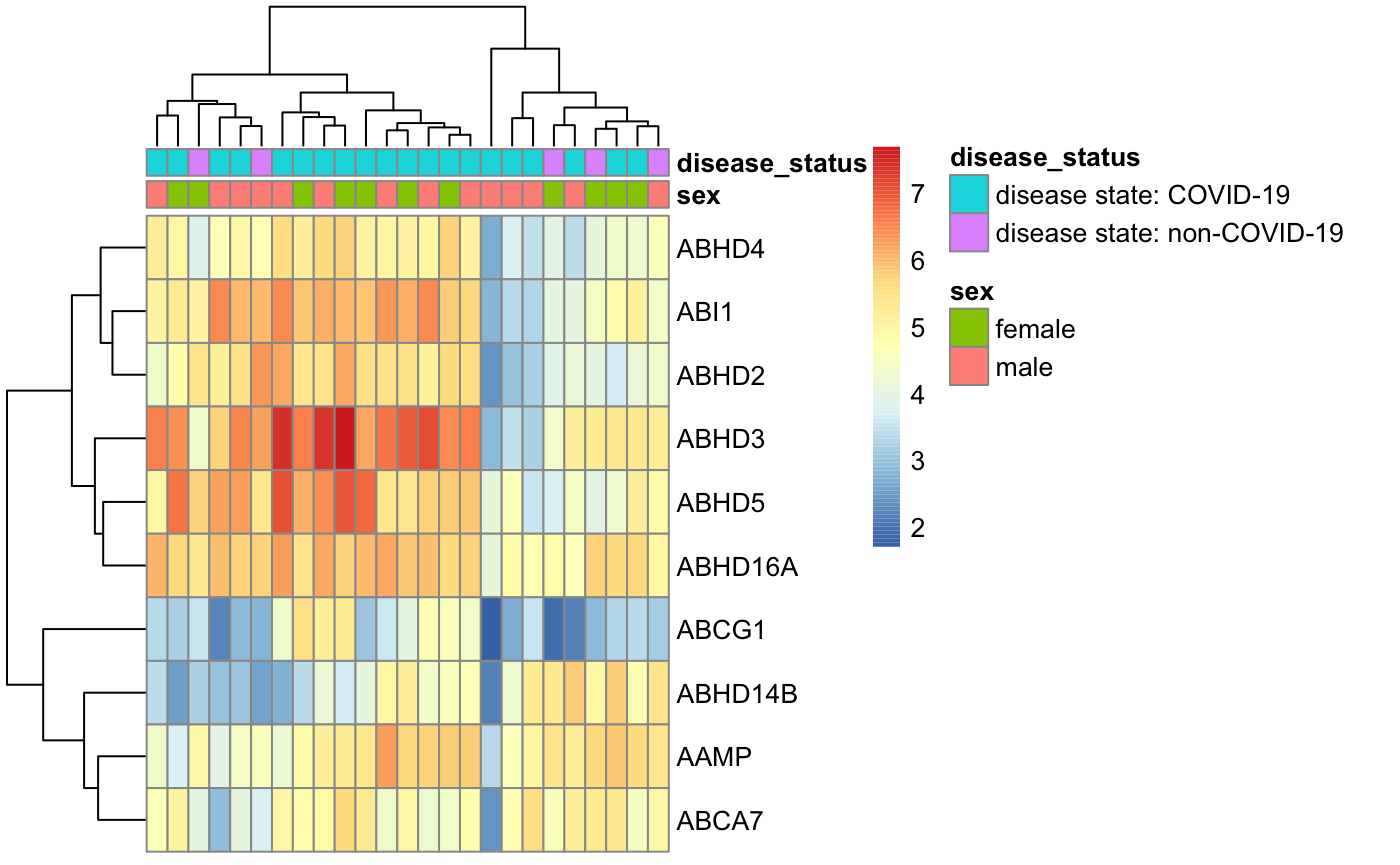
\includegraphics[width=0.80\linewidth]{heatmap.png}
\caption{\label{fig:heatmap}Heatmap of top variable genes}
\end{figure}

\subsection{2D density of AAAS expression vs. Age}

This 2D density plot shows the distribution of AAAS expression against age, stratified by COVID-19 status. In the COVID-19 group, there are visibly more samples, with most clustering in the lower-right area corresponding to older age and lower expression. However, some points show higher expression at younger ages. In the non-COVID group, the distribution is more dispersed across the plot, without a clear concentration. In conclusion, AAAS expression patterns appear more concentrated among COVID-19 patients, while non-COVID patients exhibit broader variability.

\begin{figure}[H]
\centering
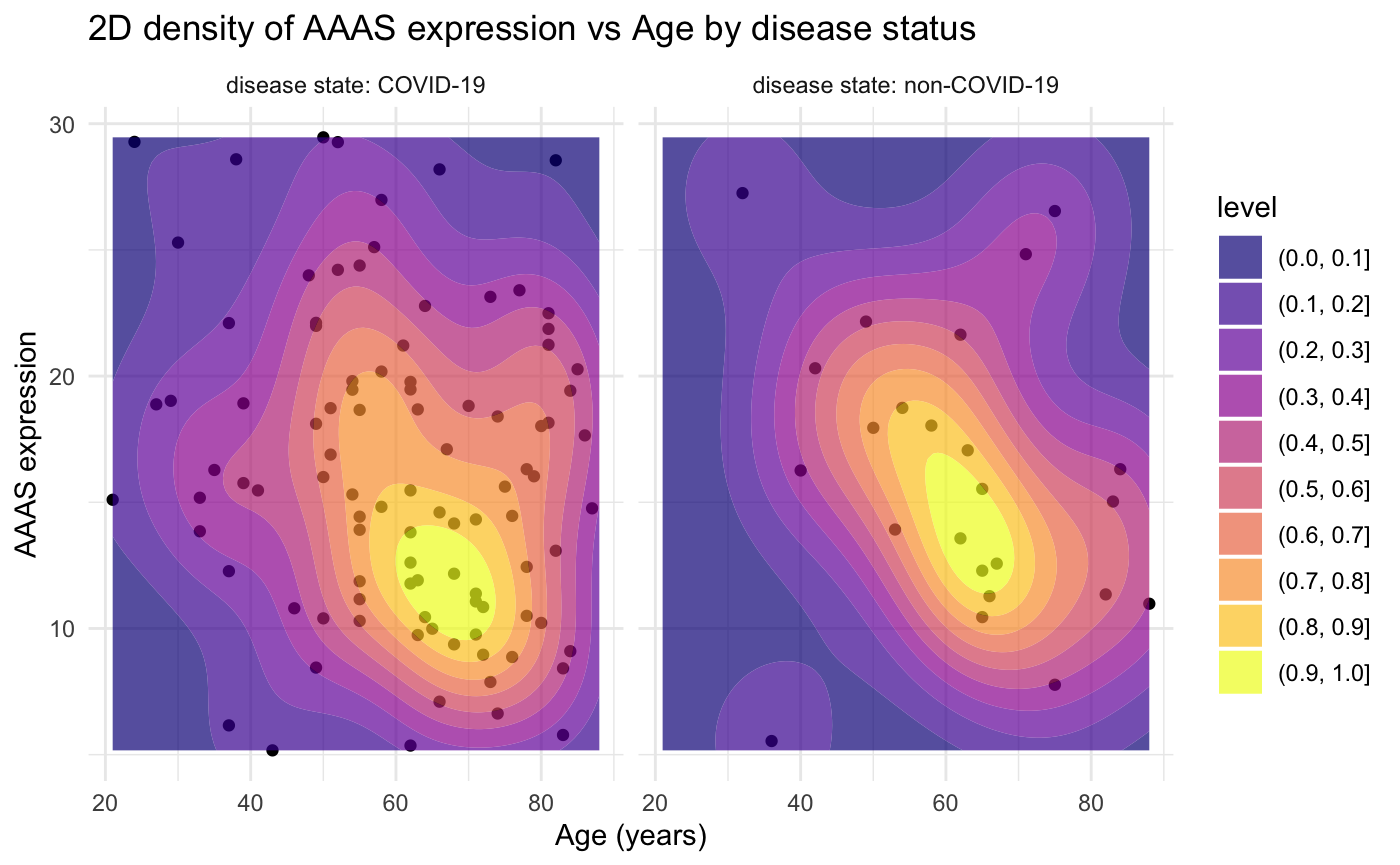
\includegraphics[width=0.80\linewidth]{2D density of AAAS expression vs Age by disease status.png}
\caption{\label{fig:2Ddensity}2D density of AAAS expression vs. Age}
\end{figure}

\subsection{Conclusion}

In summary, the analysis provides an overview of both patient characteristics and gene expression patterns. Patients with COVID-19 tend to be older, have higher ferritin levels, and more ICU admissions, suggesting a clinically more severe profile. For the AAAS gene, its expression distribution was fairly symmetric, and no strong linear relationship with age was observed. Stratification by sex and disease status indicated that neither factor alone fully explained the expression differences, though interactions may be important. The heatmap of the top variable genes showed clusters of genes with consistently low expression and others with high variability, but clustering did not clearly separate patients by COVID-19 status or sex. Finally, the 2D density plot demonstrated that COVID-19 patients were more concentrated in older age with lower AAAS expression. However, non-COVID patients had a more dispersed distribution. Together, these findings suggest that individual variability may play a larger role in gene expression differences than clinical grouping alone, and further statistical testing could help confirm these observations.

\printbibliography

\end{document}
